\documentclass[thesis.tex]{subfiles}
\begin{document}

\chapter{State of the Art}\label{chap:prevwork}

In this chapter, the most recent advancements relevant to SE on GPU and power-grid decentralization will be presented. In Section~\ref{fsea}, a fast SE approach for power grids with PMU is discussed. Section~\ref{apsse} focuses on the findings of recent research studies targeted at accelerated parallel WLS SE on CUDA. Section~\ref{ddec} presents various tested approaches for partitioning of a power grid into sectors.


\section{Fast State Estimation Algorithm }\label{fsea}
Although mathematical expressions for SE using the widely-accepted WLS algorithm at present have beneficially incorporated measurements from synchrophasors, these advancements were built on conventional network modeling approaches and computational efficiency was not of paramount importance~\cite{Huang}\cite{Gomez}.\\
Richter et al (2017)~\cite{Richter}  argue that SE computations can benefit from terminal modeling of power networks. Instead of describing or visualizing a power grid as an adjacency matrix between busses, terminal modeling enables description of the power grid using an adjacency matrix between busses and adjoining terminals in which each consecutive pair of terminals represent an edge between busses. According to Richter et al~\cite{Richter}, the terminal modeling of power networks is advantageous because of the following issues it addresses:
\begin{enumerate}
	\item Explicitness\\Terminal-modeled networks permit unique placements of RTU and PMU that is in accordance with IEC 61850-5 modeling approach for IEDs.
	\item Performance \\Slow loop-based search algorithms can be avoided because terminal modeling enables direct indexing of measurement equations and Jacobian matrices.
	\item Accuracy \\As terminal modeling offers higher level of detail in power grids, more precise estimations are possible for the system’s states.
\end{enumerate}

An example of terminal-modeled 4-bus example network is shown in Figure \ref{fig:termmod}. The adjacencies among the terminals and the busses is described using Node-terminal-incidence matrix ($\textbf{\textit{K}}_{KT}$). Similarly, the terminal admittance matrix $\textbf{\textit{Y}}_{T}$ describing the relation between the terminal voltages and current is shown in $\textbf{\textit{z}}$.
\begin{figure}[H]
	\centering
	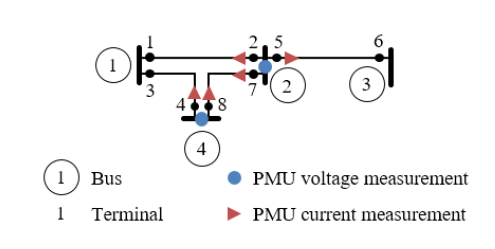
\includegraphics[scale=0.7]{termmod}
	\caption{4-bus example grid~\cite{Richter}}
	\label{fig:termmod}
\end{figure}

\begin{figure}[H]
	\centering
	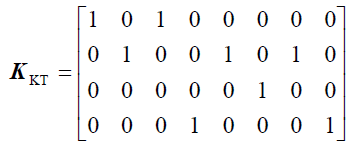
\includegraphics[scale=0.8]{kkt}
	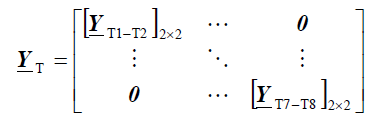
\includegraphics[scale=0.8]{yt}
	\caption*{}
\end{figure}
Using the above two matrices, the measurement functions and Jacobian matrices necessary for satisfying Equation~\ref{mainexp} can be calculated until convergence criterion is met. 
\begin{equation}\label{mainexp}
\textbf{\textit{H}}^{T}(\textbf{\textit{x}}^{k})\textbf{\textit{R}}^{-1}\textbf{\textit{H}}(\textbf{\textit{x}}^{k})(\textbf{\textit{x}}^{(k+1)}-\textbf{\textit{x}}^{k}) = \textbf{\textit{H}}^{T}(\textbf{\textit{x}}^{k})\textbf{\textit{R}}^{-1}[\textbf{\textit{z}}-\textbf{\textit{h}}(\textbf{\textit{x}}^{k})]
\end{equation}

Richter et al~\cite{Richter} have verified that this technique is especially faster for larger networks as corresponding elements may be easily accessed by the means of explicit indexing and running tedious search algorithms for finding bus numbers and measurement types can be avoided. They have also presented a strong case for inclusion of phasor measurements in the terminal-based state estimator as it significantly increases the accuracy.

\section{Accelerating SE via GPU-powered Massive Parallelization}\label{apsse}
Karimipour and Dinavahi (2013)~\cite{KarimipourAcc} have analyzed the performance impact upon using GPU’s massive parallelization for WLS State Estimation of conventionally modelled large-scale power systems. They have argued that the presence of multiple matrix-vector and matrix-matrix products in WLS method are computationally intensive. They have found that $\textbf{\textit{H}}^{T}(\textbf{\textit{x}}^{k})\textbf{\textit{R}}^{-1}\textbf{\textit{H}}(\textbf{\textit{x}}^{k})$ or $\textbf{\textit{H}}^{T}(\textbf{\textit{x}}^{k})\textbf{\textit{R}}^{-1}[\textbf{\textit{z}}-\textbf{\textit{h}}(\textbf{\textit{x}}^{k})]$ can take an order of magnitude longer execution time than that of $\textbf{\textit{R}}^{-1}[\textbf{\textit{z}}-\textbf{\textit{h}}(\textbf{\textit{x}}^{k})]$. Similarly, profiling of operation $\textbf{\textit{G}}(\textbf{\textit{x}})\delta(\textbf{\textit{x}}) = \textbf{\textit{g}}(\textbf{\textit{x}})$ has shown that it is very expensive due to the large size of the required inverse matrix computation. In their research for acceleration, Karimipour et al~\cite{KarimipourAcc} have offloaded all arithmetic operations to the CUDA kernels on the GPU as can be also observed in Figure~\ref{fig:karimipour}. As shown, after acquisition of the measurement vector $\textbf{\textit{z}}$ and the covariance matrix $\textbf{\textit{R}}$, the datasets are transferred to the GPU followed by arithmetic computations being carried out on the GPU.
\begin{figure}[H]
	\centering
	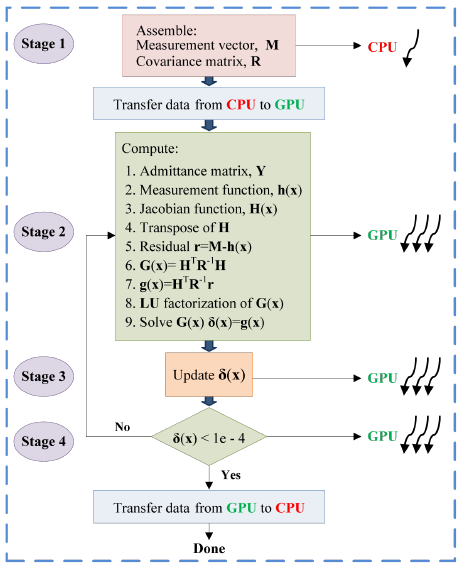
\includegraphics[scale=0.8]{karimipour}
	\caption{GPU implementation of WLS algorithm~\cite{KarimipourAcc}}
	\label{fig:karimipour}
\end{figure}
In order to avoid direct computation of $\textbf{\textit{G}}(\textbf{\textit{x}})^{-1}$ for solving $\delta(\textbf{\textit{x}})$, LU decomposition is performed using cuBLAS library. Upon testing with networks of various sizes ranging from 39-bus to 4992-bus using an NVIDIA Fermi GPU (512 CUDA cores, 256 FP64 GFLOPS) against an Intel Xeon E5-2620 (6-core, 2.0 GHz, 32GB RAM), they recorded performance speedups up to 38 times against serial execution on CPU.

\section{Domain Decomposition for SE in Power Grids}\label{ddec}
With increase in size, inclusion of PMU data and a need for higher monitoring resolution for safe administration of the power grid, new faster techniques have been developed in order to minimize computational burden~\cite{Xiong}\cite{Muscas}\cite{KarimipourDec}. Such techniques have been sought after since as early as 1995~\cite{Falcao} and have enabled parallel and distributed computation with low communication costs. \\
Domain decomposition techniques is one of these techniques and is used to partition a power grid into a set of several smaller subsystems or sectors that can be processed and solved separately through parallel processing on multiprocessors. \\
The two major approaches for domain decomposition are:
\begin{enumerate}
	\item Overlapping subdomains.
	\item Non-overlapping subdomains.
\end{enumerate}
Xiong and Grijalva~\cite{Xiong} have studied non-overlapping automatic grid partitioning using standard graph partitioning toolbox METIS. According to them, a power system is equivalent to an undirected graph and therefore should have 3 desirable properties when subjected to decomposition to permit decentralized SE:
\begin{enumerate}
	\item The number of busses in every partition should be nearly equal leading to nearly equal number of states. Due to this, it can expected that computation times across multiple partitions are approximately close and larger partitions which can result in processing bottlenecks can be avoided.
	\item The number of lines that traverse the partitions should be as low as possible. 
	\item Each partition of the grid must be locally ‘fully observable’.
\end{enumerate}
A power grid is fully-observable when voltage and phases at all the busses can be uniquely estimated using the available measurements. For $\Delta \textbf{\textit{x}} = (\textbf{\textit{H}}^{T}\textbf{\textit{R}}^{-1}\textbf{\textit{H}})^{-1}\textbf{\textit{H}}^{T}\textbf{\textit{R}}^{-1}\Delta \textbf{\textit{z}}$, $\Delta \textbf{\textit{x}}$ can be calculated if $\textbf{\textit{H}}^{T}\textbf{\textit{R}}^{-1}\textbf{\textit{H}}$ is non-singular or if $\textbf{\textit{H}}$ has a full column rank. The observability of a partition depends on the number of measurements available; Xiong and Grijalva~\cite{Xiong} have in their simulations ensured the observability by including sufficient number of measurements at the finest granularity of partitions, i.e. every bus. This however is not applicable in practice.\\\\
Similarly, Karimipour and Dinavahi~\cite{KarimipourDec} have successfully analysed the application of non-overlapping decomposition using Additive Schwarz Method (ASM) which reduces the execution time by splitting relatively similar amount of work among many processors. It is applicable for large scale systems with speedup in the range of 4-6 times.. In their study, large-scale SE case studies up to the size of 4992-bus power system were constructed by duplicating IEEE 39-bus system and interconnecting them together.\\\\
An overlapping decomposition approach has been adopted by Muscas et al~\cite{Muscas} as shown in Figure~\ref{fig:mdsse}. According to them, apart from the aforementioned 3 desirable properties and an overlapping node, the overlapping node must be “fully monitored through a suitable measurement point”. ‘Multi-area DSSE’ algorithm proposed by them consists of a two-step process. At first, local estimation (BC-DSSE) is done in each sub-area which results in a set of branch currents and nodal voltages. Upon completion, this is followed by a fast estimation harmonization (second WLS step) of results exploiting the border(overlapping bus) information.

\begin{figure}[H]
	\centering
	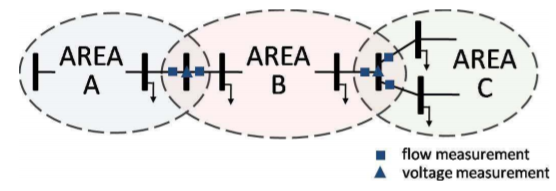
\includegraphics[scale=0.8]{mdsse}
	\caption{Multi-area network division scheme~\cite{Muscas}}
	\label{fig:mdsse}
\end{figure}



\subfilebib % Makes bibliography available when compiling as subfile
\end{document}